%Ne pas numéroter cette partie
\part*{Annexes}
%Rajouter la ligne "Annexes" dans le sommaire
\addcontentsline{toc}{part}{Annexes}

\section{Quelques informations sur la démographie de la zone}

Valérie Delaunay, nous a produit un export de la base de données de l'observatoire de Niakar pour la commune de Diohine. Cela nous a permit de produire les deux graph de la figure \ref{fig:obsNiakhar}

\begin{figure}
     \centering
     \begin{subfigure}[b]{0.45\textwidth}
         \centering
         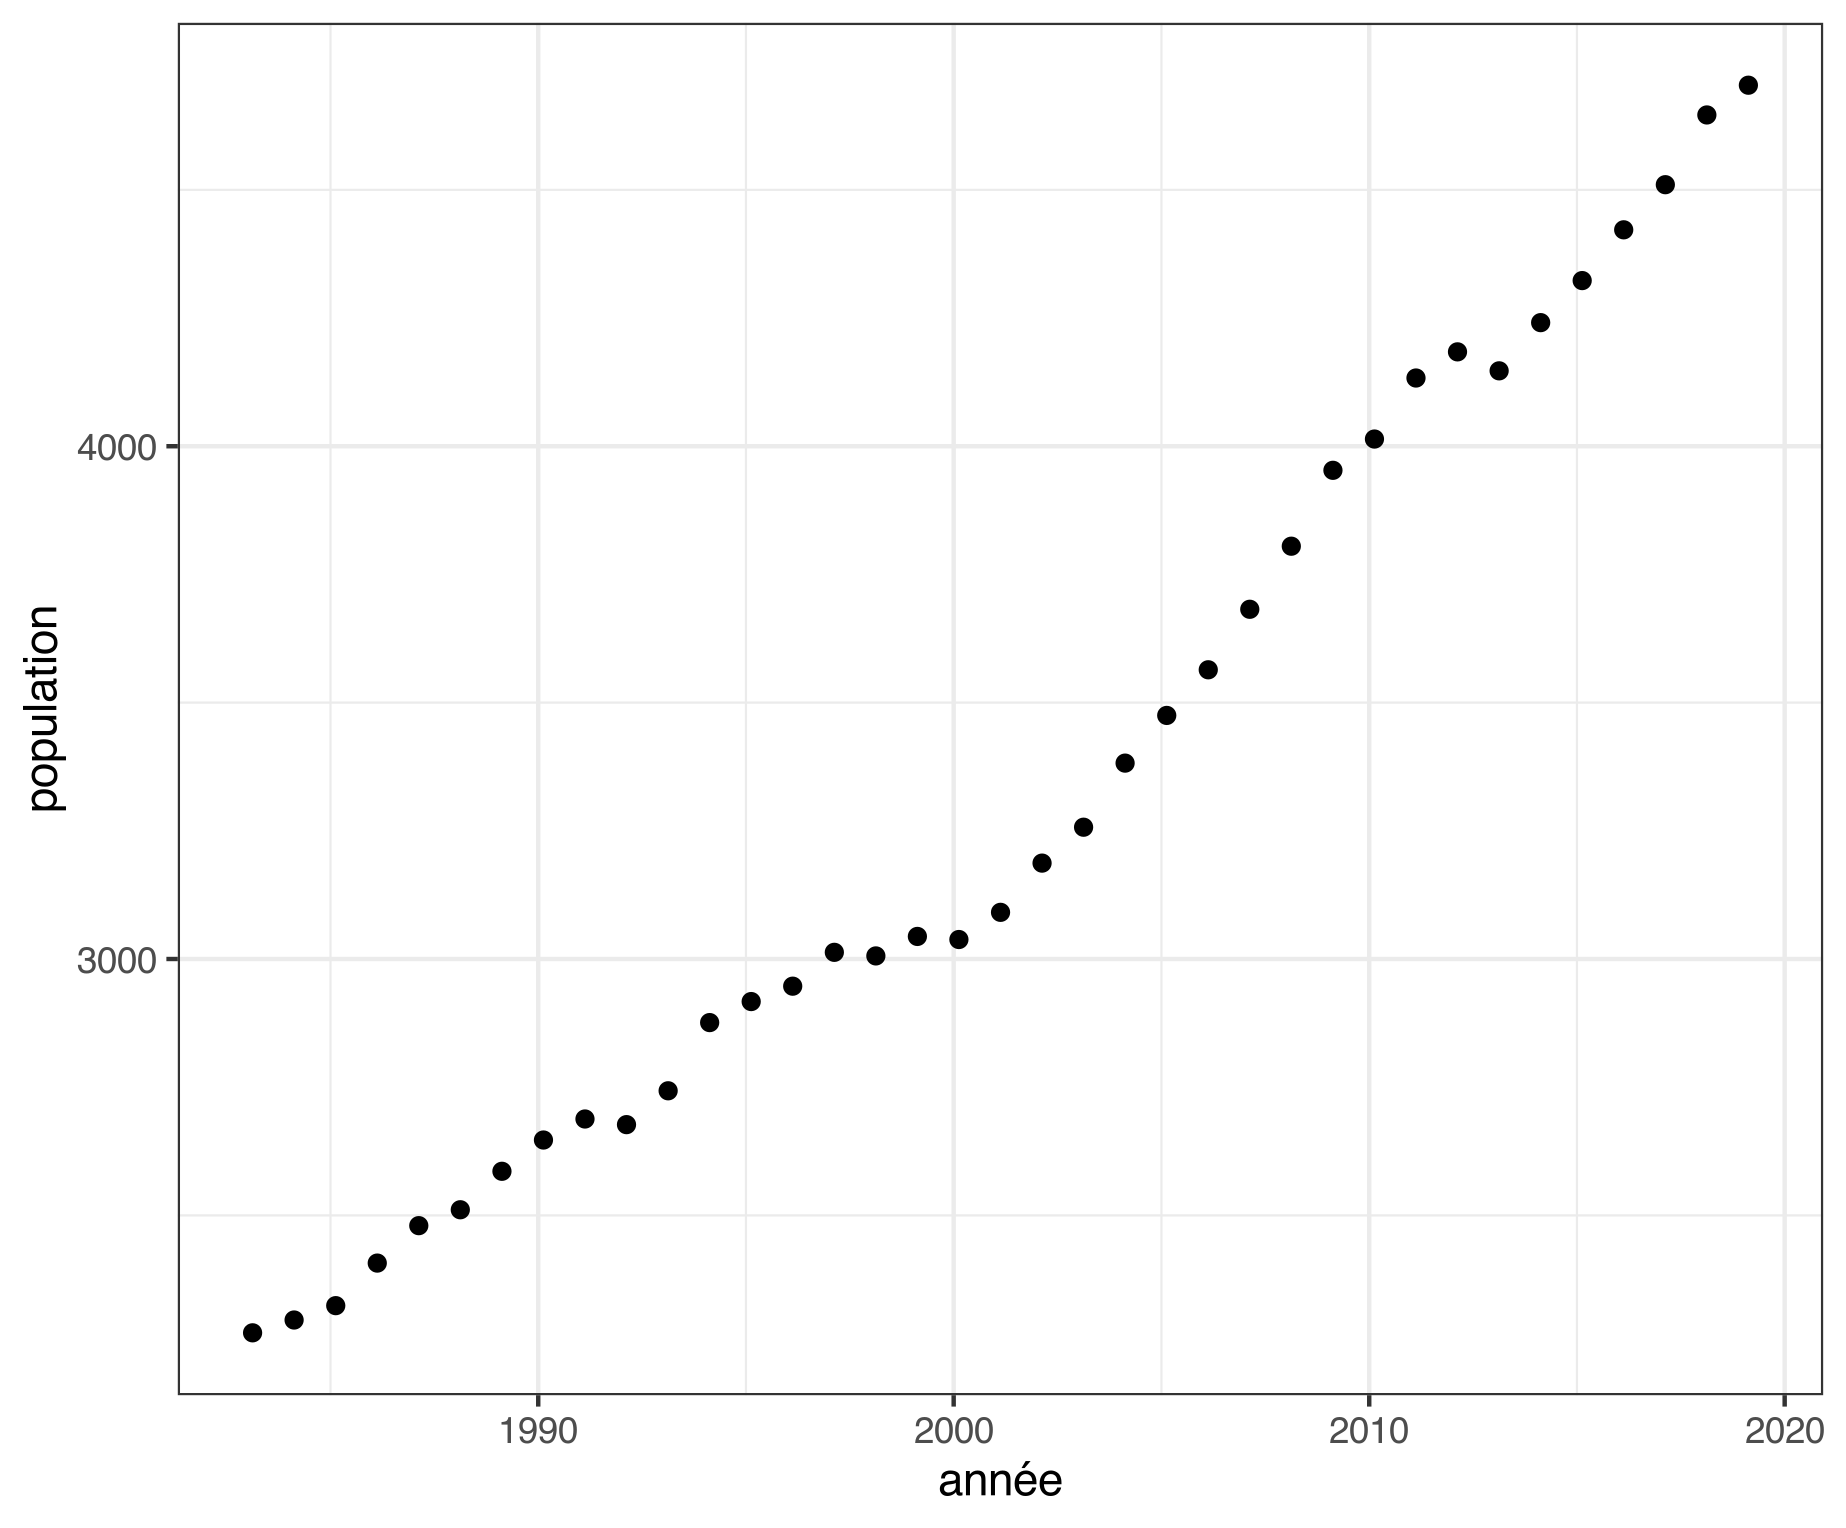
\includegraphics[width=\textwidth]{img/population1995-2020_diohine.png}
         \caption{$y=x$}
         \label{fig:pop}
     \end{subfigure}
     \hfill
     \begin{subfigure}[b]{0.45\textwidth}
         \centering
         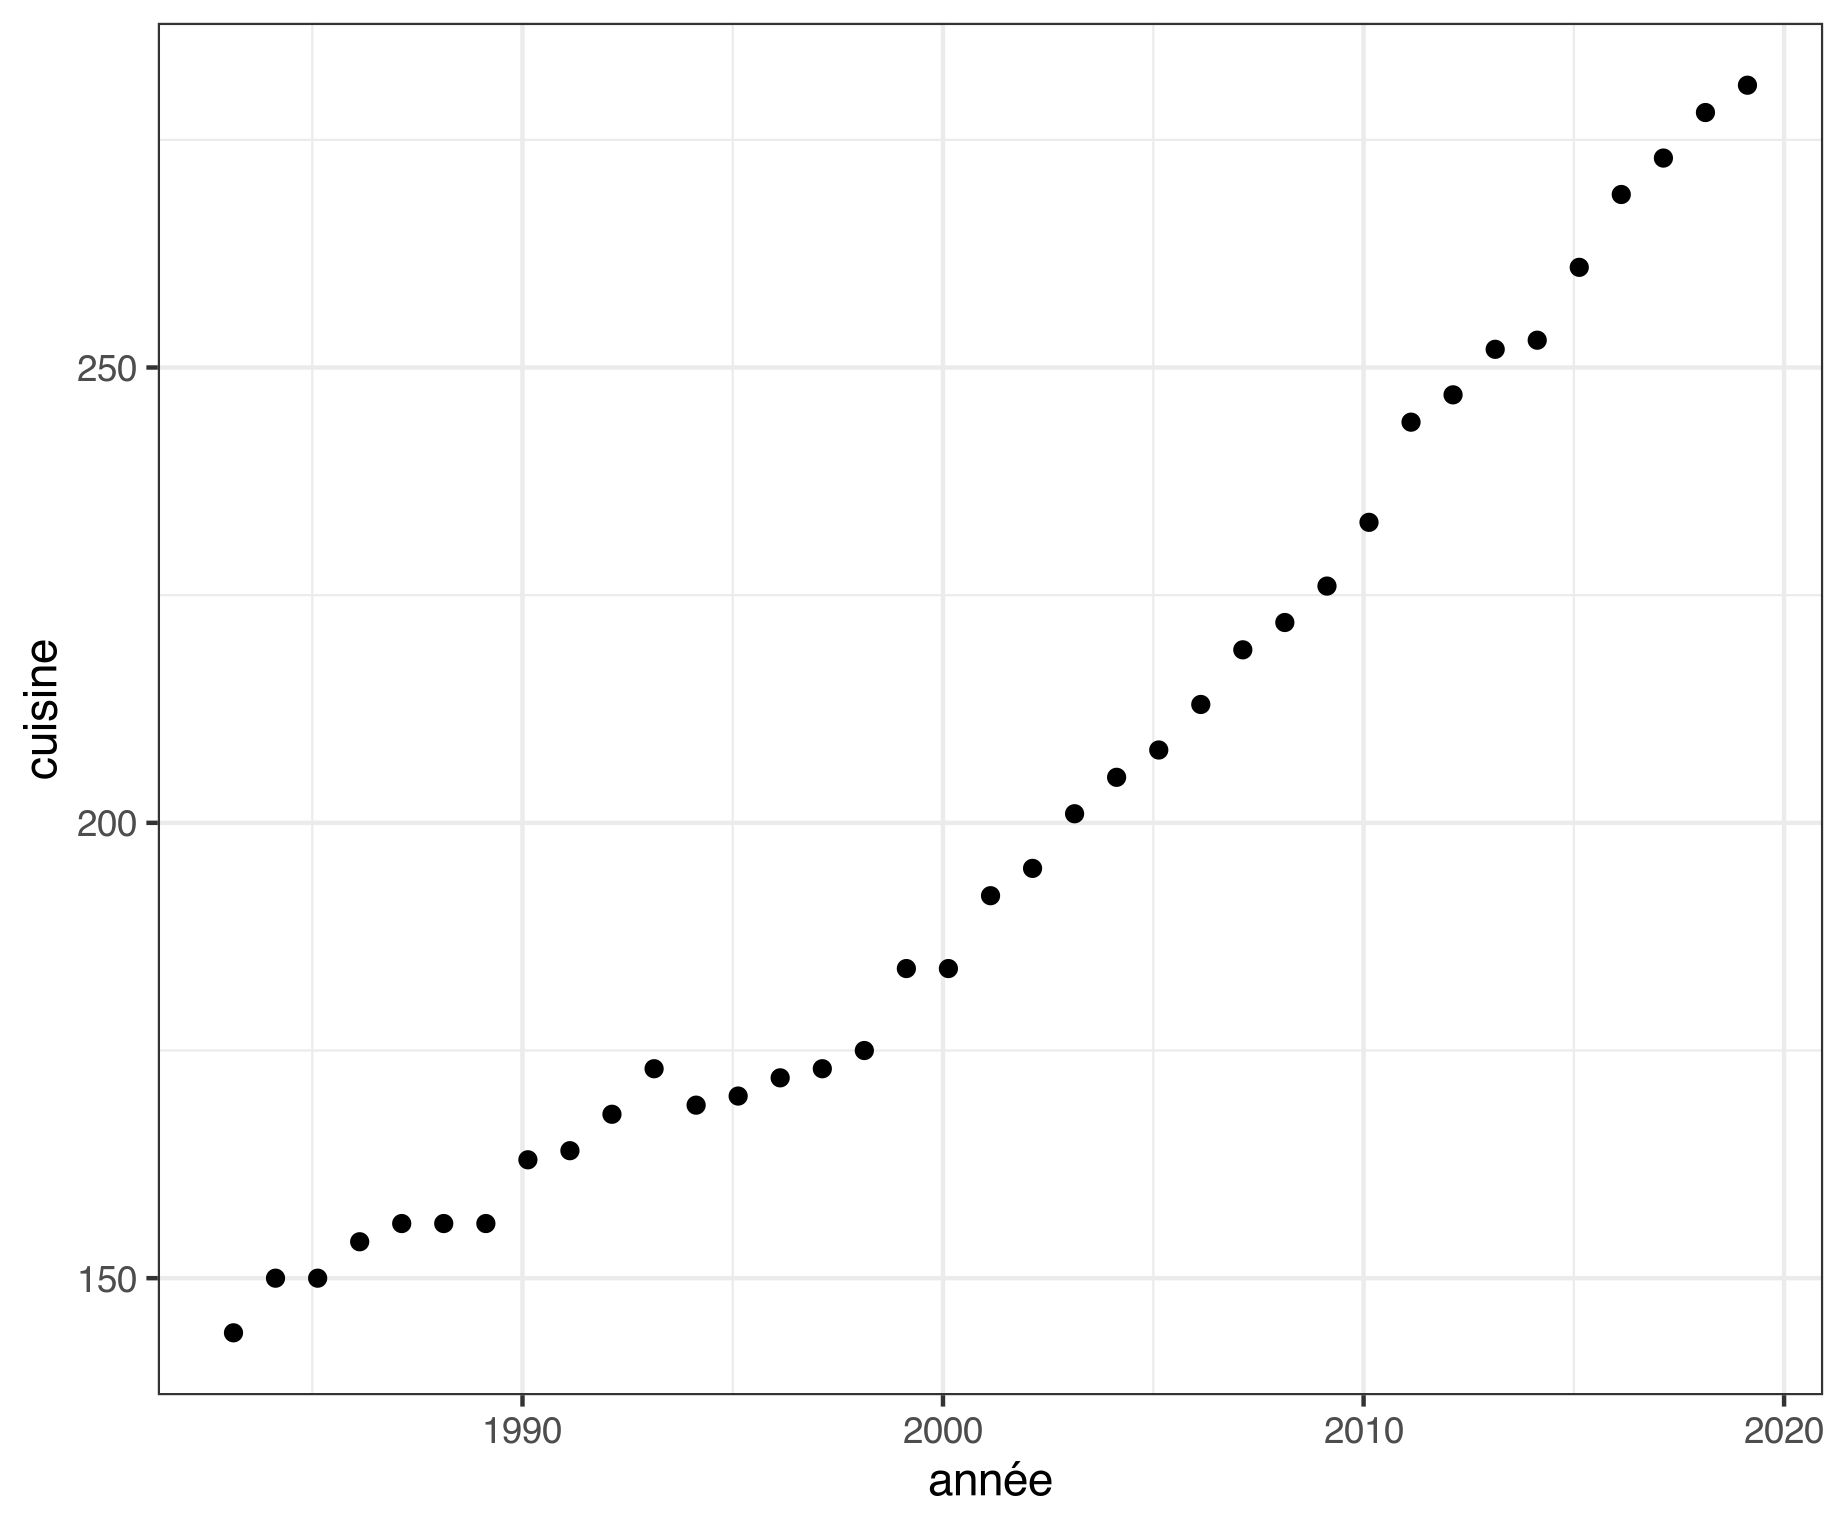
\includegraphics[width=\textwidth]{img/cuisine1995-2020_diohine.png}
         \caption{$y=3sinx$}
         \label{fig:cuisines}
     \end{subfigure}
        \caption{Données de l'observatoire de Niakar entre 1985 et 2020. la fig \subref{fig:pop} représente l'évolution de la population, la fig. \subref{fig:cuisines} montre l'évolution du nombre de cuisine sur la même période.}
        \label{fig:obsNiakhar}
\end{figure}

On a calcule donc les valeurs du tableau \ref{tab:obsNiakhar}.

  \begin{table}[]
    \begin{center}
      \begin{tabular}{ll}
      \hline
      Accroissement par ans (ln)                                                               & 67,99 \\ \hline
      \begin{tabular}[c]{@{}l@{}}Nombre moyen de personnes\\ par cuisines\end{tabular}         & 16,52 \\ \hline
      \begin{tabular}[c]{@{}l@{}}Ecart type du nombre de \\ personne par cuisines\end{tabular} & 0,54  \\ \hline
      \end{tabular}
      \caption{Tableau des valeurs calculer à partir des données de l'observatoire de Niakhar}
      \label{tab:obsNiakhar}
    \end{center}
  \end{table}


\section{Les grandes lignes de l'usage de DOT}

Dans le cadre des atelier, nous avons également utiliser un formalisme de description de graph issue de la librairie graphviz sous forme de $.dot$ . On peut donc conserver de point les graph sous une forme manipulable avec des outils informatique.

\begin{itemize}
  \item ouvrir le .dot dans R avec le package sna $\longrightarrow$ enregistrer en $.gv$ on l'ouvre tout seul dans Rstudio.
  %[La doc de rendu est pas mal](https://rich-iannone.github.io/DiagrammeR/graphviz_and_mermaid.html)
  \item enrichir le graphe avec des attributs dans R ou à la main dans le fichier en utilisant la synthaxe de DiagrammR. par exemple `@@1` pour définir un attribut
  \item visualiser avec diagrammeR
  \item Pour le rendu : utilisation de la substitution de diagrammeR pour changer les couleurs les formes etc.  des noeuds et des arêtes
\end{itemize}

Paul à rédiger un script qui est disponible (comme les données) sur github.

\subsection{ Le workflow}
\begin{itemize}
  \item Defintion de class de noeud
  \item Extrait les sous graph avec igraph
  \item enrichissemement des attribut du graph genre color etc.
  \item renvoyer en `.gv`
\end{itemize}



\section{quelques notes et idées}

On regroupe ici quelques idées qui n'ont pas encore trouver leur place dans le rapport.


Les lois en droit positif on l'oublie trop souvent servent à maintenir la paix sociale.

Spinoza pose en effet qu'il suffit de ne pas comprendre pour moraliser. Et c'est ce à quoi servent les lois. À gérer les problèmes des gens qui ne veulent pas comprendre. "Si Adam ne comprend pas la règle du rapport de son corps avec le fruit, il entend la parole de Dieu comme une défense. Bien plus, la forme confuse de la loi morale a tellement compromis la loi de la nature que la philosophie ne doit pas parler de loi de la nature, mais seulement de vérité éternelles "  p. 35, "les lois morale ou sociale ne nous apportent aucune connaissance, elle ne fait rien connaitre". Au pire elle empêche la formation de la connaissance (loi des tyrans). Au mieux elle prépare la connaissance et la rend possible (loi d'Abraham). Entre ces deux extrêmes, elle supplée à la connaissance chez ceux qui n'en sont pas capables en raison de leurs modes d'existence (loi de moise)."
>[name= Etienne] J'ai l'impression que tout le système traditionnel à Diohine est tourné vers une résolution de conflit où la seule chose qui est donnée aux acteurs c'est des indications de posture (tu ne dois pas faire de tort... $\longrightarrow$ injonction morale/ethique $\longrightarrow$ ligne de conduite serere), Donc on les pousse à comprendre la source du conflict (mauvais de Spinoza)parce qu'il y a une injonction a l'action (une action de réparation).

Changement de plan/d'arène juridique : Quand ils ne sont pas parvenus à une résolution locale du conflit, on entre dans le droit positif (dur et sans empathie $\longrightarrow$ paul Sene) et là il y a des lois qui font qu'on a plus besoin de comprendre le source du mauvais. $\longrightarrow$ un lien avec un verbatim en \href{https://hackmd.openmole.org/qhPAjsJGRbiOQYIItbwPww#J4---21-octobre}{J4} "Tout le processus est là pour éviter la dureté des lois. “\textit{au niveau du sous-préfet, il n’y a plus de sentiments, c’est la légalité dans toute sa froideur}”"

\begin{quote}
  >[name= Paul] Ne pas vouloir qu'on casse la paix sociale ça veux pas dire qu'on cherche a la maintenir. Les mécanismes d'exclusion, sont une réaction au comportement délétère et pas une proaction en faveur de son épanouissement. La loi intervient "en négatif" pour se débarasser de ce qui met à mal la paix sociale. Une question pour Philippe Karpe : le capital de paix sociale est il croissant par nature ?

  >[name= Etienne] Quand une personne va en brousse, c'est pour se faire oublier donc la paix social
\end{quote}

La théorie de l'économie des conventions [boltanski et thévenot]  semble bien adaptée pour lire la paix sociale de Diohine: (source wikipedia) Celui-ci part de l'idée que pour qu'il y ait échange, coordination, coopération entre des agents, il faut qu'il y ait des *conventions* entre les personnes concernées ; c’est-à-dire un \textit{système d'attentes réciproques} entre les personnes sur leurs comportements.

ces attentes peuvent être dans au moins trois cités : la cité domestique , cité civique et peut être cité par projets dans une moindre mesure pour des décision ponctuelles : orientation spcéifique après la première chasse, creuser un puits, établir une banque etc. avec les acteurs qui ne sont pas agro pasteurs\\
Ca sera surtout utile pour la gestion des conflits avec les différents niveaux de la colonnes de spération du conflit  cf la page wikipedia : Il survient une controverse dans une même cité. Pour la clore, on recourt à un principe supérieur commun. Car les personnes engagées dans une même cité ont un même système d'équivalence, ils se déplacent dans une grandeur identique. Les objets sont identifiés et hiérarchisés de manière compatible.

Il peut coexister des cités différents sans discordes. Mais dans ce cas l'équilibre reste provisoire. Il peut survenir un différend entre des cités. La discorde doit, pour être clarifiée, être rapportée à une cité et une seule. Elle peut également être résolue par un arrangement, les partenaires se mettent localement d'accord sur une transaction. Enfin, les acteurs peuvent arriver à un compromis, et dans ce cas, ils réunissent plusieurs cités à travers un bien commun.\footnote{source : \url{ https://www.cnam.fr/servlet/com.univ.collaboratif.utils.LectureFichiergw?ID_FICHIER=1295877017868}}
